\section{Causal Impact Analysis}
Before conducting our primary text mining analysis, we first establish the causal impact of ChatGPT on Stack Overflow question volumes. This section outlines our causal inference methodology and findings, which provide critical context for interpreting the subsequent textual analysis results.

%%%%%%%%%%%%%%%%%%%%%%%%%%%%%%%%%%%%%%%%%%%%%%%%%%%%%%%%%%%%%%%%%%%%%%%%%%%%%%%%%%%%%%%%%%%%%%%%

\subsection{Synthetic Difference-in-Differences Methodology}
To identify the causal impact of ChatGPT on Stack Overflow question volumes, we employ a Synthetic Difference-in-Differences (SDID) approach (\cite{arkhangelsky_synthetic_2021}). This methodology combines the strengths of traditional difference-in-differences and synthetic control methods, allowing us to construct a credible counterfactual for Stack Overflow in the absence of ChatGPT.\\

The selection of Mathematics, Physics, Superuser, and AskUbuntu as control units was strategically motivated by several considerations. First, these Stack Exchange forums represent technical knowledge domains with structured question patterns similar to Stack Overflow, yet they address distinct subject matters that were less effectively handled by early ChatGPT versions. While ChatGPT demonstrated strong capabilities in programming tasks from its initial release, it exhibited notable limitations in advanced mathematics, physics reasoning, and system-specific troubleshooting—areas central to our control forums. Second, these forums maintain sufficient question volumes to provide statistical power while exhibiting pre-treatment correlation with Stack Overflow question patterns (cf. \figureref{fig:correlation_matrix}), suggesting similar responsiveness to seasonal trends and external factors affecting forum usage.\\

A critical assumption for traditional difference-in-differences analysis is the parallel trends assumption, which requires that treatment and control groups would follow similar trajectories in the absence of treatment. While examining raw counts shows substantial scale differences between forums, log transformation reveals approximately parallel pre-treatment trends, particularly for scripting language questions (cf. Figure \ref{fig:paralleL_trend_trans}). This transformation addresses heterogeneity in question volumes and improves the validity of our causal inference by better satisfying the parallel trends assumption.\\

\begin{figure}[H]
    \centering
    \includesvg[width=1\linewidth]{imgs/indexed_trends.svg}
    \caption{Parallel trends: Weekly raw vs indexed question counts}
    \label{fig:paralleL_trend_trans}
\end{figure}

Despite the similar pre-treatment trends, concerns remain about external shocks that might differentially affect Stack Overflow and control forums. Our methodological approach addresses this in two complementary ways. First, our baseline DiD implementation using Stata's \mintinline{stata}{xtdidregress} automatically adjusts for both panel (forum) effects and time effects in calculating the treatment effect. We verified the robustness of these results by explicitly testing specifications with additional time fixed effects at various granularities (weekly, monthly, quarterly), which yielded identical treatment effect estimates.\\

Second, our synthetic DiD approach further strengthens causal identification by constructing a weighted combination of control units that better approximates the counterfactual for Stack Overflow. This method implicitly accounts for time-varying factors to the extent they similarly affect both treatment and control units, creating a more credible counterfactual than standard DiD approaches relying solely on parallel trends assumptions. Together, these approaches provide robust evidence that our findings reflect the causal impact of ChatGPT rather than coincidental time-specific shocks.

%%%%%%%%%%%%%%%%%%%%%%%%%%%%%%%%%%%%%%%%%%%%%%%%%%%%%%%%%%%%%%%%%%%%%%%%%%%%%%%%%%%%%%%%%%%%%%%%

\subsubsection{Model Specification}
Our base difference-in-differences (DiD) model can be expressed as:

\begin{equation}\label{eq:basedid}
\ln(Q_{it}) = \beta_1(Treatment_i \times Post_t) + \gamma_i + \lambda_t + \varepsilon_{it}
\end{equation}

where $\ln(Q_{it})$ represents the log-transformed question count for forum $i$ at time $t$, $\text{Treatment}_i$ is an indicator for Stack Overflow (being 1 in the case of Stack Overflow and 0 otherwise), $\text{Post}_t$ is an indicator for periods after ChatGPT's release (November 30, 2022, being 1 after and 0 otherwise).  Furthermore, $\gamma_i$ represents forum fixed effects, $\lambda_t$ represents time fixed effects, and $\varepsilon_{it}$ is the error term. Lastly, the coefficient $\beta_1$ captures the average treatment effect on the treated (ATET) - the causal impact of ChatGPT on Stack Overflow question volume.\\

For our synthetic DiD approach, we follow \textcite{arkhangelsky_synthetic_2021}, where the estimator can be expressed as:

\begin{equation}\label{eq:synthdid}
\hat{\tau}_{\text{SDID}} = \sum_{t=T_0+1}^T \lambda_t \left( Y_{1t} - \sum_{j=2}^J \omega_j Y_{jt} \right) - \sum_{t=1}^{T_0} \lambda_t \left( Y_{1t} - \sum_{j=2}^J \omega_j Y_{jt} \right)
\end{equation}

where $Y_{jt}$ represents the log-transformed question count for forum $j$ at time $t$, $\omega_j$ are unit weights, $\lambda_t$ are time weights, $T_0$ is the last pre-treatment period, and unit $j=1$ represents Stack Overflow. We implemented this methodology using \textcite{clarke_synthetic_2023, ciccia_short_2024}'s Stata implementation to ensure robustness of our findings, and conducted both static SDID analysis and dynamic event study specifications.

%%%%%%%%%%%%%%%%%%%%%%%%%%%%%%%%%%%%%%%%%%%%%%%%%%%%%%%%%%%%%%%%%%%%%%%%%%%%%%%%%%%%%%%%%%%%%%%%

\subsection{Causal Impact Results}

%%%%%%%%%%%%%%%%%%%%%%%%%%%%%%%%%%%%%%%%%%%%%%%%%%%%%%%%%%%%%%%%%%%%%%%%%%%%%%%%%%%%%%%%%%%%%%%%

\subsubsection{Base DiD Estimates}
We begin with standard DiD estimates for both all Stack Overflow questions and specifically for scripting language questions (JavaScript, Python, R, and PHP). Table \ref{tab:did_results} presents these base DiD results, while Table \ref{tab:sdid_results} presents the synthetic DiD estimates with and without covariate controls.

\begin{table}[H]
    \centering
    \caption{Basic DiD Estimates of ChatGPT's Impact on Stack Overflow Question Volume}
    \label{tab:did_results}
    \begin{tabular}{lcc}
        \toprule
            & \multicolumn{2}{c}{Dependent variable: Log Question Count} \\
            \cmidrule(lr){2-3}
            & All Questions & Scripting Languages \\
        \midrule
            Treatment Effect & $-0.241^{***}$ & $-0.443^{***}$ \\
            & $(0.034)$ & $(0.054)$ \\
        \midrule
            Time fixed effects & Yes & Yes \\
            Group fixed effects & Yes & Yes \\
            Percent Change & $-21.4\%$ & $-35.8\%$ \\
        \midrule
            Observations & 830 & 1,328 \\
            Number of groups & 5 & 8 \\
            Pre-treatment periods & 101 & 101 \\
            Post-treatment periods & 65 & 65 \\
        \bottomrule
            \multicolumn{3}{p{0.95\linewidth}}{\footnotesize \textit{Notes:} Standard errors in parentheses, clustered by forum/group. $^{***}p<0.001$. The dependent variable is log question count. Treatment is defined as the period after ChatGPT's release (November 30, 2022).} \\
    \end{tabular}
\end{table}

These results indicate statistically significant negative effects across all model specifications. For all Stack Overflow questions, the standard DiD model (Table \ref{tab:did_results}) indicates a 21.4\% decrease in question volume, while the synthetic DiD models (Table \ref{tab:sdid_results}, columns 1-2) suggest a larger 26.7\% reduction. For scripting language questions, we observe a much larger decline of 35.8\% in the standard DiD model and 39.5\% in the synthetic DiD model. This differential impact suggests that ChatGPT has been particularly effective at addressing programming questions related to these popular scripting languages.

%%%%%%%%%%%%%%%%%%%%%%%%%%%%%%%%%%%%%%%%%%%%%%%%%%%%%%%%%%%%%%%%%%%%%%%%%%%%%%%%%%%%%%%%%%%%%%%%

\subsubsection{Synthetic DiD Results}
To address potential violations of the parallel trends assumption and create a more credible counterfactual, we employ the SDID approach. Figure \ref{fig:sdid_all} visualizes the results for all Stack Overflow questions, while Figure \ref{fig:sdid_script} focuses on scripting language questions, and Table \ref{tab:sdid_results} presents the formal SDID estimates.

\begin{figure}[H]
    \centering
    \begin{subfigure}[b]{0.475\textwidth}
        \centering
        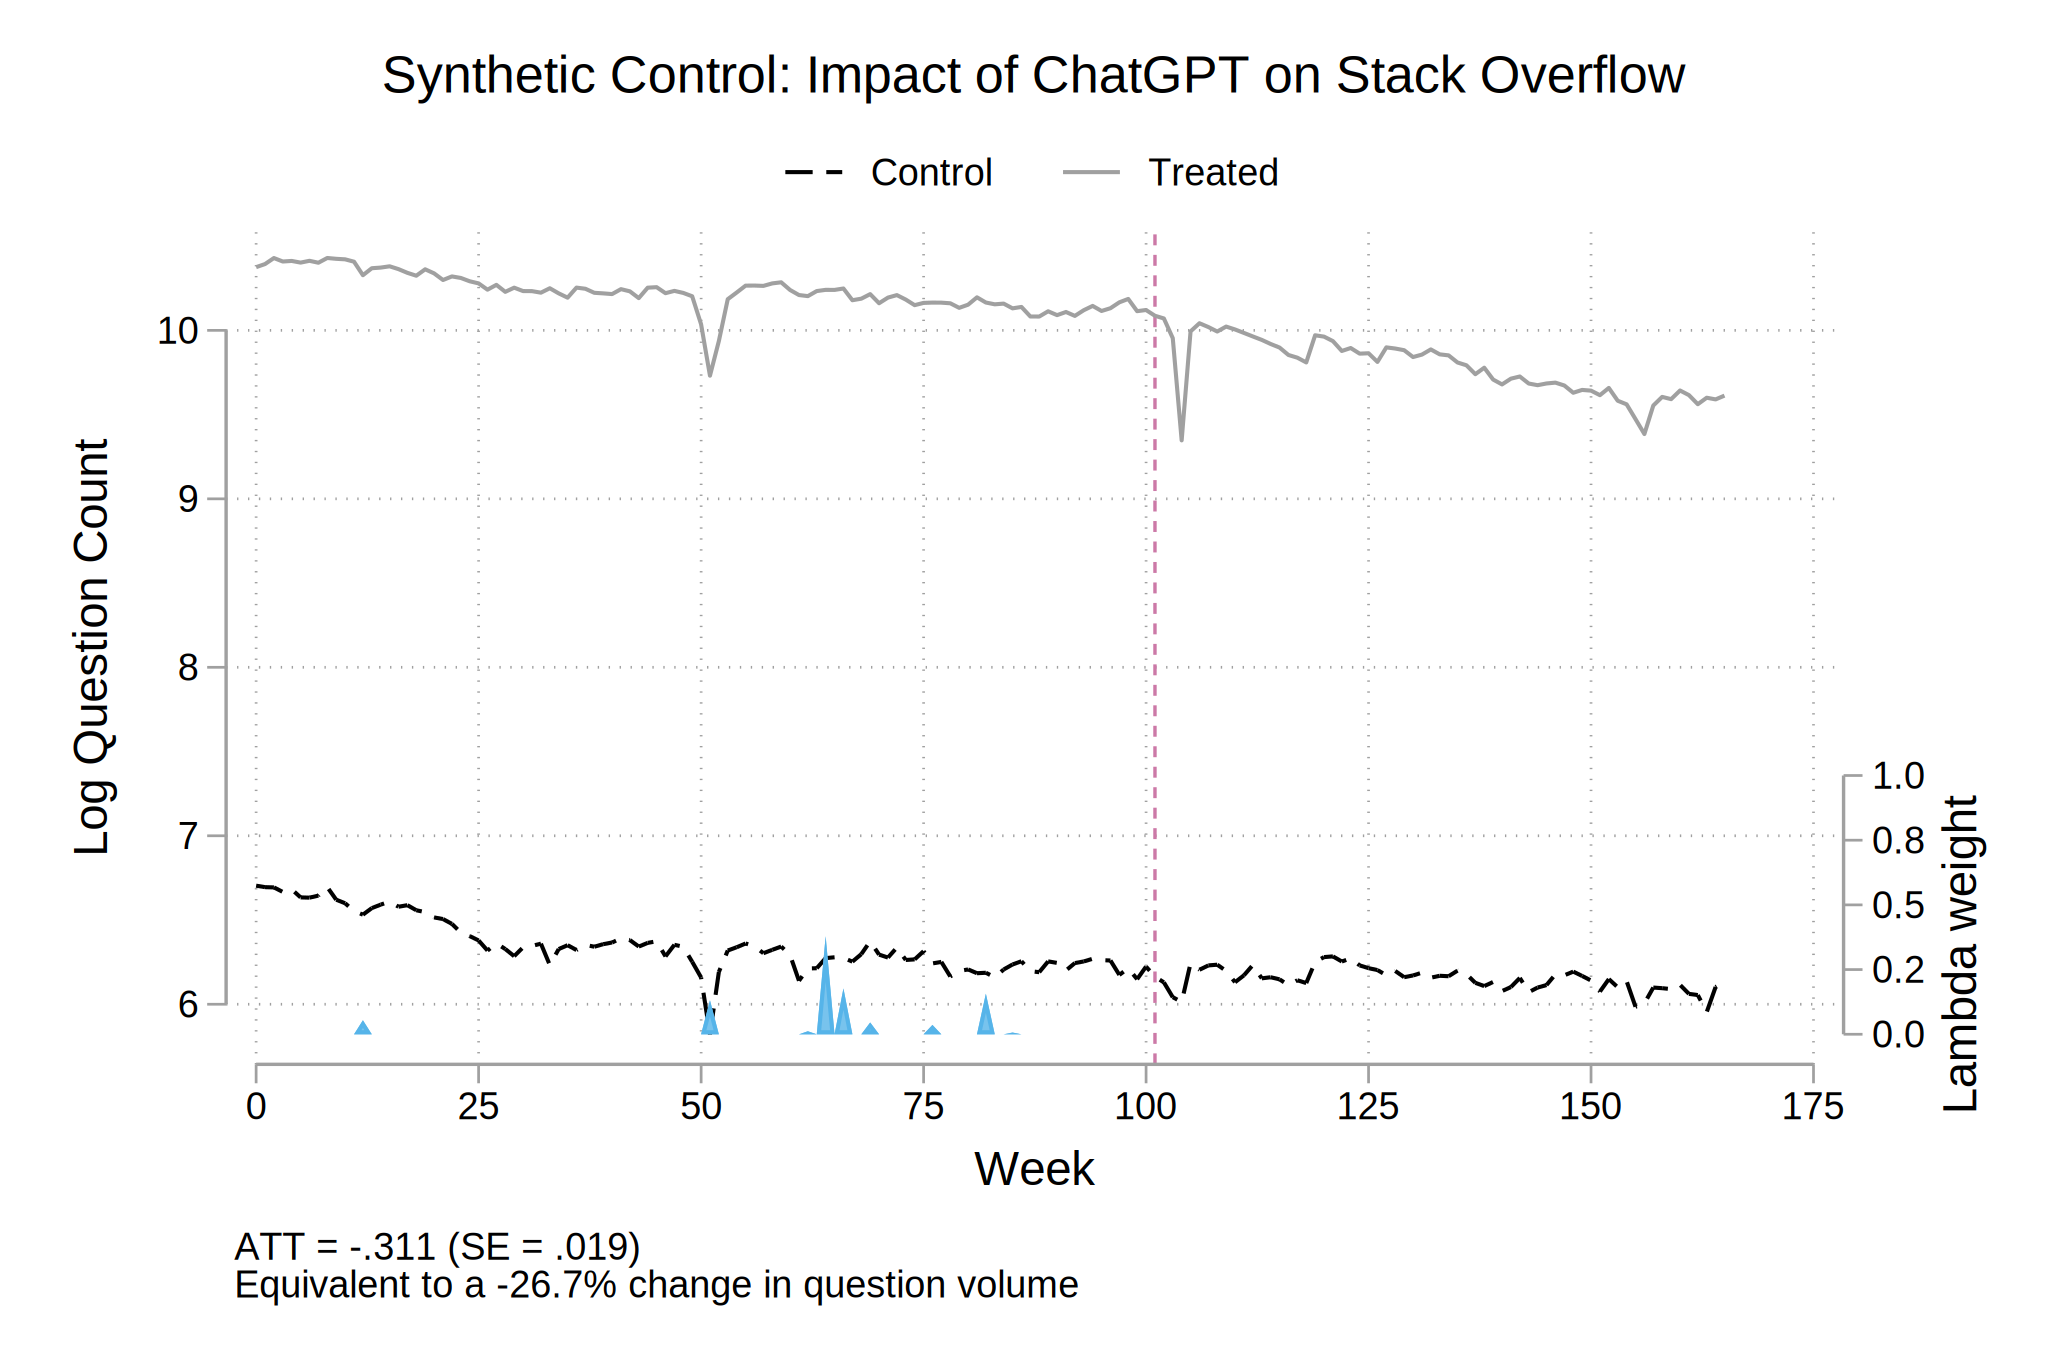
\includegraphics[width=1\textwidth]{imgs/stata/sdid_all_trends101.pdf}
        \caption{Impact on All Stack Overflow Questions}
        \label{fig:sdid_all}
    \end{subfigure}
    \hfill
    \begin{subfigure}[b]{0.475\textwidth}
        \centering
        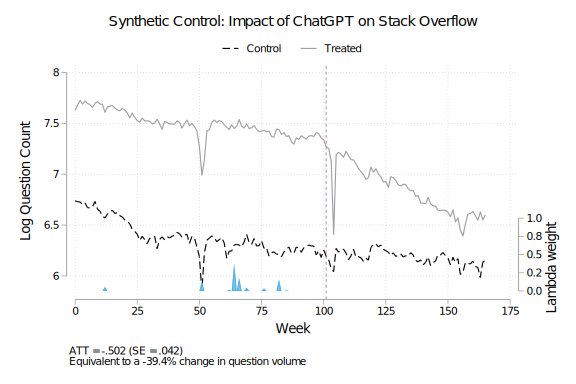
\includegraphics[width=1\textwidth]{imgs/stata/sdid_script_trends101.pdf}
        \caption{Impact on Scripting Language Questions}
        \label{fig:sdid_script}
    \end{subfigure}
    \caption{Synthetic difference-in-difference plots}
    \label{fig:DiD}
\end{figure}

\begin{table}[H]
    \centering
    \caption{Synthetic DiD Estimates of ChatGPT's Impact on Stack Overflow Question Volume}
    \label{tab:sdid_results}
    \begin{tabular}{lcccc}
        \toprule
            & \multicolumn{2}{c}{All Questions} & \multicolumn{2}{c}{Scripting Languages} \\
            \cmidrule(lr){2-3} \cmidrule(lr){4-5}
            & (1) & (2) & (3) & (4) \\
        \midrule
            Treatment Effect & $-0.311^{***}$ & $-0.308^{***}$ & $-0.502^{***}$ & $-0.497^{***}$ \\
            & $(0.019)$ & $(0.000)$ & $(0.042)$ & $(0.039)$ \\
        \midrule
            Month covariates & No & Yes & No & Yes \\
            Percent Change & $-26.7\%$ & $-26.5\%$ & $-39.5\%$ & $-39.2\%$ \\
        \midrule
            Observations & 830 & 830 & 1,328 & 1,328 \\
            Number of groups & 5 & 5 & 8 & 8 \\
            Pre-treatment periods & 101 & 101 & 101 & 101 \\
            Post-treatment periods & 65 & 65 & 65 & 65 \\
        \bottomrule
            \multicolumn{5}{p{0.95\linewidth}}{\footnotesize \textit{Notes:} Standard errors in parentheses based on placebo/bootstrap replications (100 repetitions). $^{***}p<0.001$. The dependent variable is log question count. All models include time and group fixed effects. Treatment is defined as the period after ChatGPT's release (November 30, 2022).} \\
    \end{tabular}
\end{table}

The SDID approach yields larger treatment effect estimates compared to standard DiD, suggesting that the traditional DiD may underestimate the impact. The SDID results indicate a 26.7\% reduction in overall question volume and a substantial 39.5\% reduction in scripting language questions (covariate-adjusted results are 26.5\% and 39.2\% respectively).

%%%%%%%%%%%%%%%%%%%%%%%%%%%%%%%%%%%%%%%%%%%%%%%%%%%%%%%%%%%%%%%%%%%%%%%%%%%%%%%%%%%%%%%%%%%%%%%%

\subsubsection{Event Study Analysis}
We conduct a synthetic event study analysis to explore how the treatment effect evolved over time, following \textcite{ciccia_short_2024}. Unlike standard event study approaches, the synthetic difference-in-differences (SDID) event study estimator can be expressed as:

\begin{equation}
    \hat{\tau}^{sdid}_{\ell} = \sum_{a \in A_{\ell}} \frac{N^a_{tr}}{N^{\ell}_{tr}} \hat{\tau}^{sdid}_{a,\ell}
\end{equation}

where $\hat{\tau}^{sdid}_{a,\ell}$ represents the dynamic treatment effect $\ell$ periods after treatment for cohort $a$:

\begin{equation}
    \hat{\tau}^{sdid}_{a,\ell} = \frac{1}{N^a_{tr}} \sum_{i \in I^a} Y_{i,a-1+\ell} - \sum_{i=1}^{N_{co}} \omega_i Y_{i,a-1+\ell} - \sum_{t=1}^{a-1} \left( \frac{1}{N^a_{tr}} \sum_{i \in I^a} \lambda_t Y_{i,t} - \sum_{i=1}^{N_{co}} \omega_i \lambda_t Y_{i,t} \right)
\end{equation}

In our application, $Y_{it}$ is the log-transformed question count for forum $i$ at time $t$, with the different programming languages on Stack Overflow as the treated units (corresponding to $I^a$). The weights $\omega_i$ and $\lambda_t$ are optimally chosen to create a synthetic control that best approximates Stack Overflow's pre-treatment outcome trajectory. For each relative time period $\ell$, the estimator compares the difference between actual and synthetic outcomes to their pre-treatment average difference.

\begin{figure}[H]
    \centering
    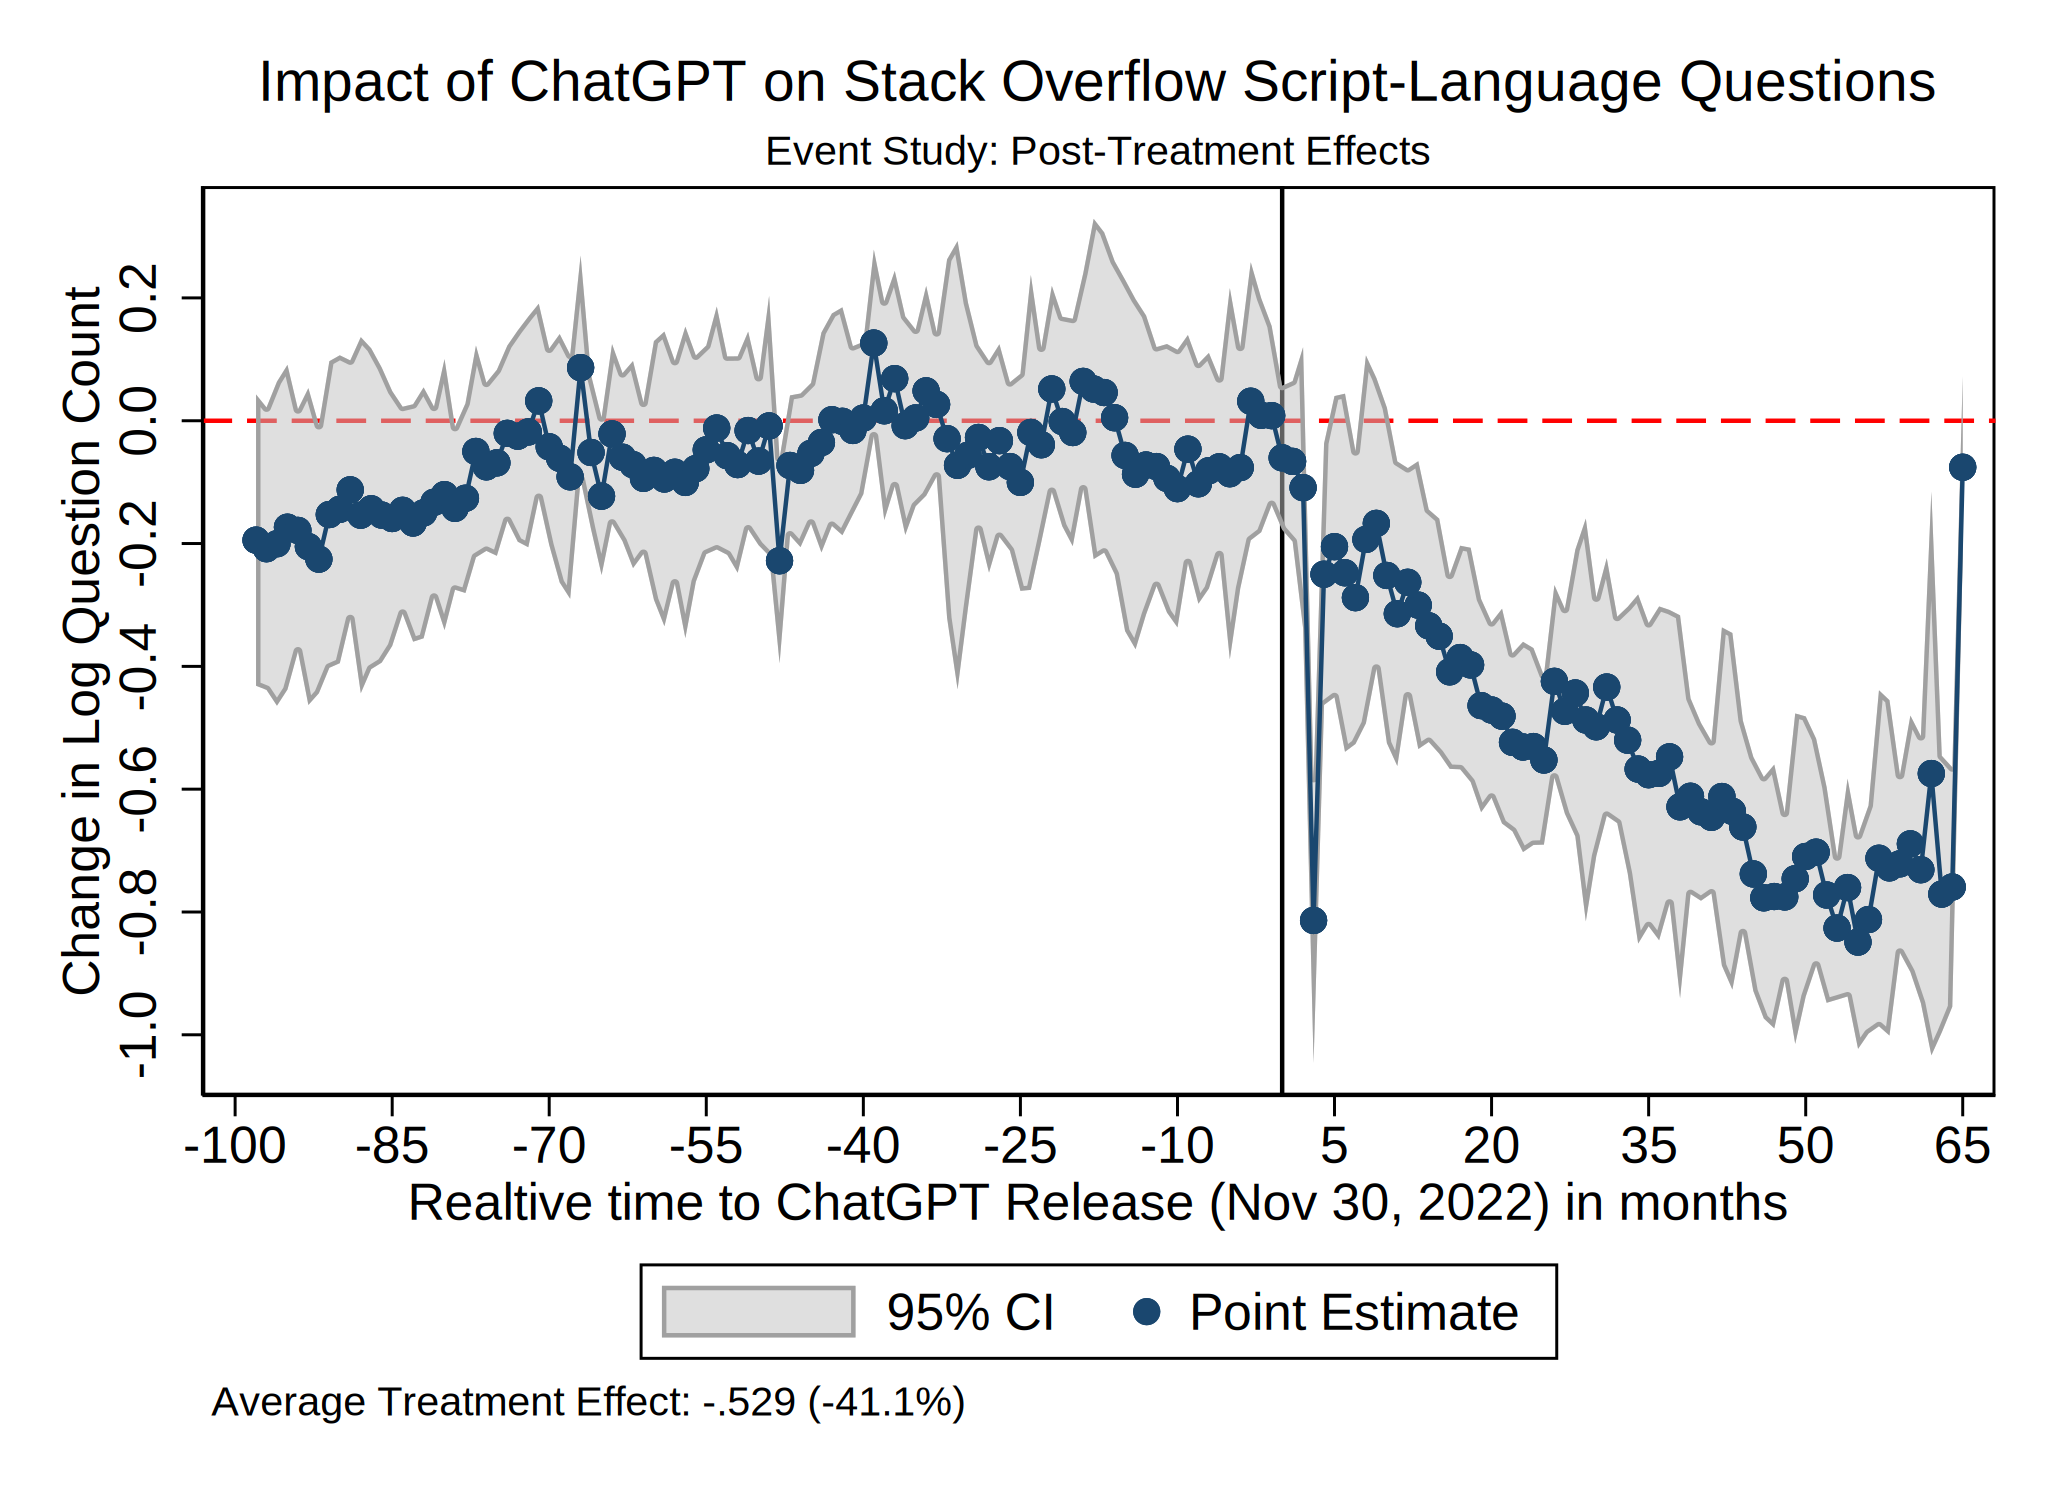
\includegraphics[width=0.9\textwidth]{imgs/stata/event_study_scripting_languages.pdf}
    \caption{Event Study Analysis for Scripting Language Questions}
    \label{fig:event_study}
\end{figure}


This approach allows us to examine treatment effects at specific time points relative to ChatGPT's release (November 30, 2022), with $\ell < 0$ for pre-treatment periods and $\ell > 0$ for post-treatment periods. By implementing this within the synthetic DiD framework, each relative time coefficient is estimated using the synthetic control method, comparing Stack Overflow to a weighted combination of control forums optimized for that specific time period. Figure \ref{fig:event_study} displays the results for scripting language questions, and Table \ref{tab:event_study_results} presents the event study estimates across different time periods.

\begin{table}[H]
    \centering
    \caption{Event Study: Post-Treatment Effects Over Time for Scripting Languages}
    \label{tab:event_study_results}
    \begin{tabular}{lccc}
    \toprule
    Time Period & Estimate & SE & 95\% CI \\
    \midrule
    Week 1-4 after treatment   & -0.335 & 0.079 & [-0.490, -0.180] \\
    Week 5-12 after treatment  & -0.267 & 0.084 & [-0.432, -0.102] \\
    Week 13-24 after treatment & -0.482 & 0.080 & [-0.639, -0.325] \\
    Week 25-36 after treatment & -0.577 & 0.082 & [-0.738, -0.416] \\
    Week 37-48 after treatment & -0.644 & 0.077 & [-0.795, -0.493] \\
    Week 49-60 after treatment & -0.718 & 0.081 & [-0.877, -0.559] \\
    Week 61-65 after treatment & -0.739 & 0.077 & [-0.890, -0.588] \\
    \midrule
    Overall treatment effect & -0.502 & 0.073 & [-0.646, -0.358] \\
    \bottomrule
    \multicolumn{4}{p{0.95\linewidth}}{\footnotesize \textit{Notes:} Results from synthetic DiD event study analysis with bootstrapped standard errors (100 repetitions). Estimates show the change in log question count for Stack Overflow scripting language questions relative to the synthetic control group across different post-treatment time periods. All effects are statistically significant at the 0.1\% level.} \\
    \end{tabular}
\end{table}

The event study reveals several important patterns: (1) An immediate and substantial drop in question volume following ChatGPT's release. (2) Persistence of the effect throughout the post-treatment period. (3) Intensification of the effect over time, with the most recent period showing the strongest effect, suggesting continued adoption of ChatGPT for programming assistance.

%%%%%%%%%%%%%%%%%%%%%%%%%%%%%%%%%%%%%%%%%%%%%%%%%%%%%%%%%%%%%%%%%%%%%%%%%%%%%%%%%%%%%%%%%%%%%%%%

\subsection{Robustness and Potential Confounders}

The stability of our estimates across different model specifications provides strong evidence of robustness. Adding monthly covariates yields nearly identical treatment effects for both all questions (-0.308 vs. -0.311) and scripting languages (-0.497 vs. -0.502). While our methodology addresses many potential confounders, some limitations remain: (1) concurrent AI tool releases may have contributed to the observed effects, such as the introduction and evolution of GitHub Copilot; (2) despite controlling for time-invariant forum characteristics and common shocks, forum-specific trends could still influence results; and (3) potential spillover effects may exist if users reduced activity across multiple Stack Exchange forums after discovering ChatGPT. Despite these considerations, the magnitude, immediacy, and persistence of effects—particularly for scripting languages—strongly suggest a causal relationship between ChatGPT's introduction and the decline in Stack Overflow question volume.

%%%%%%%%%%%%%%%%%%%%%%%%%%%%%%%%%%%%%%%%%%%%%%%%%%%%%%%%%%%%%%%%%%%%%%%%%%%%%%%%%%%%%%%%%%%%%%%%

\subsection{Implications for Text Analysis}

These findings establish a causal impact of ChatGPT on Stack Overflow question volumes, particularly for scripting language questions. The differential impact on scripting languages (approximately 39\% reduction compared to 27\% overall) suggests that ChatGPT has been particularly effective at addressing common programming queries.

This causal foundation motivates our core research question: How has the nature of the remaining questions changed? The dramatic reduction in volume indicates a fundamental shift in how developers seek programming assistance. Still, it raises important questions about the characteristics of questions that continue to be asked on Stack Overflow despite the availability of ChatGPT. Our subsequent text mining analysis will identify and quantify these changes in question content, complexity, and topical focus.